\documentclass[conference]{IEEEtran}
\IEEEoverridecommandlockouts

\usepackage{cite}
\usepackage{amsmath}
\usepackage{amssymb}
\usepackage{amsfonts}
\usepackage{algorithm}
\usepackage{algpseudocode}
\usepackage{graphicx}
\usepackage{textcomp}
\usepackage{hyperref}
\usepackage{tabularx}
\usepackage{caption}
\usepackage{subcaption}

\graphicspath{/images}

\title{Online Polycube Packing with Deep Reinforcement Learning\\
\thanks{This thesis was prepared in partial fulfillment of the requirements for the Degree of Bachelor of Science in Data Science and Artificial Intelligence, Maastricht University. Supervisor: Dr. Thomas Bitterman}
}

\author{\IEEEauthorblockN{Thomas Vroom}
\IEEEauthorblockA{\textit{Department of Advanced Computing Sciences} \\
\textit{Faculty of Science and Engineering}\\
\textit{Maastricht University}\\
Maastricht, The Netherlands}
}

\begin{document}
\maketitle

%
% ABSTRACT
%
\begin{abstract}
    In this thesis we investigate the performance of deep reinforcement learning in solving the online polycube packing problem, a variant of online 3D bin packing that uses polycubes as items.
    We compare the performance of deep reinforcement learning to traditional packing heuristics in terms of the number of polycubes packed and the time it took to pack them, and investigate if the performance of deep reinforcement learning can be improved by using heuristics to restrict the action space.
    Our results show that Proximal Policy Optimization (PPO) together with invalid action masking can successfully solve the online polycube packing problem, and is on average faster than traditional packing heuristics.
    However, an optimal set of heuristics will on average still be able to pack more polycubes than a deep reinforcement learning agent.
    We also find that restricting the action space using heuristics does not necessarily lead to better performance, but does greatly increase the training time of PPO.
    Our findings suggest that deep reinforcement learning is a valid approach for solving online polycube packing problems, but more research is needed to improve the overall performance.
\end{abstract}

\begin{IEEEkeywords}
    Packing Problems, Polycubes, Deep Reinforcement Learning, Proximal Policy Optimization, Action Masking
\end{IEEEkeywords}

%
% Introduction
%
\section{Introduction} \label{sec:introduction}
Bin Packing Problems (BPP) are some of the most popular and well-studied combinatorial optimization problems.
The standard 1D Bin Packing Problem (1D-BPP) seeks to pack a set of items of varying weights into a minimum number of bins with a fixed capacity: a classic NP-hard problem \cite{Korte2012}.
In higher dimensions the problem is often simplified by only using a single bin with fixed dimensions, where items are represented as geometric shapes \cite{Salih2023}.
Traditionally, BPP assumes that all items to be packed are known a priori, which is referred to as offline BPP \cite{Martello1998}.
However, in many real-world applications items arrive sequentially, and it is not always possible to move items once they have been placed in the container.
This variation is known as online BPP, and is considered harder because of the limited information available \cite{Seiden2001}.

Out of all the BPP variants, online 3D-BPP, a variant where items are represented as simple 3D shapes like cuboids, is considered one of the most practically useful \cite{Martello1998}\cite{Zhao2022pct}.
The more general variant, online 3D-BPP with irregular shapes, has been studied less, even though it is even more relevant to real-world applications \cite{Zhao2022general}.
A likely reason for this is because the step from simple 3D shapes to irregular shapes is a significant leap in complexity \cite{Zhao2022general}.
In this thesis, we consider the online polycube packing problem: a variant of online 3D-BPP that uses polycubes as items.
Polycubes are a generalization of polyominoes to three dimensions: connected sets of unit cubes in 3D space (see Figure \ref{fig:polycubes}) \cite{WeissteinPolycube}.

\begin{figure}[!htb]
    \centering
    \begin{subfigure}[b]{0.3\textwidth}
        \centering
        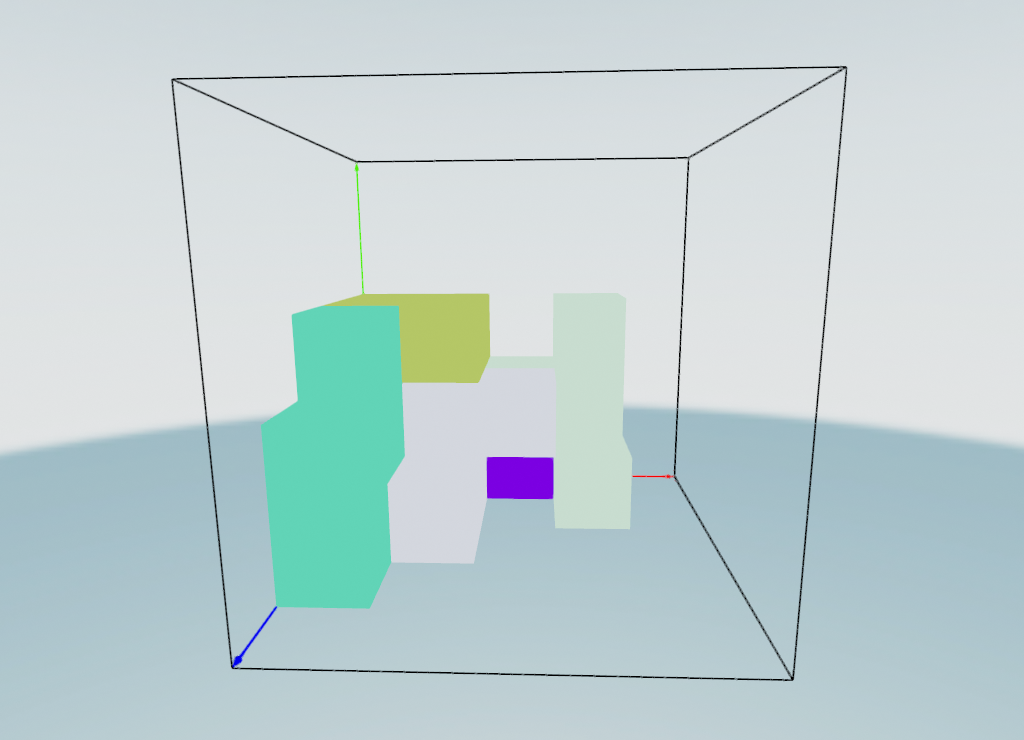
\includegraphics[width=0.95\textwidth]{images/blbf.png}
        \caption{Bottom-Left-Back-Fill (BLBF).}
        \label{fig:blbf}
    \end{subfigure}
    \hfill
    \begin{subfigure}[b]{0.3\textwidth}
        \centering
        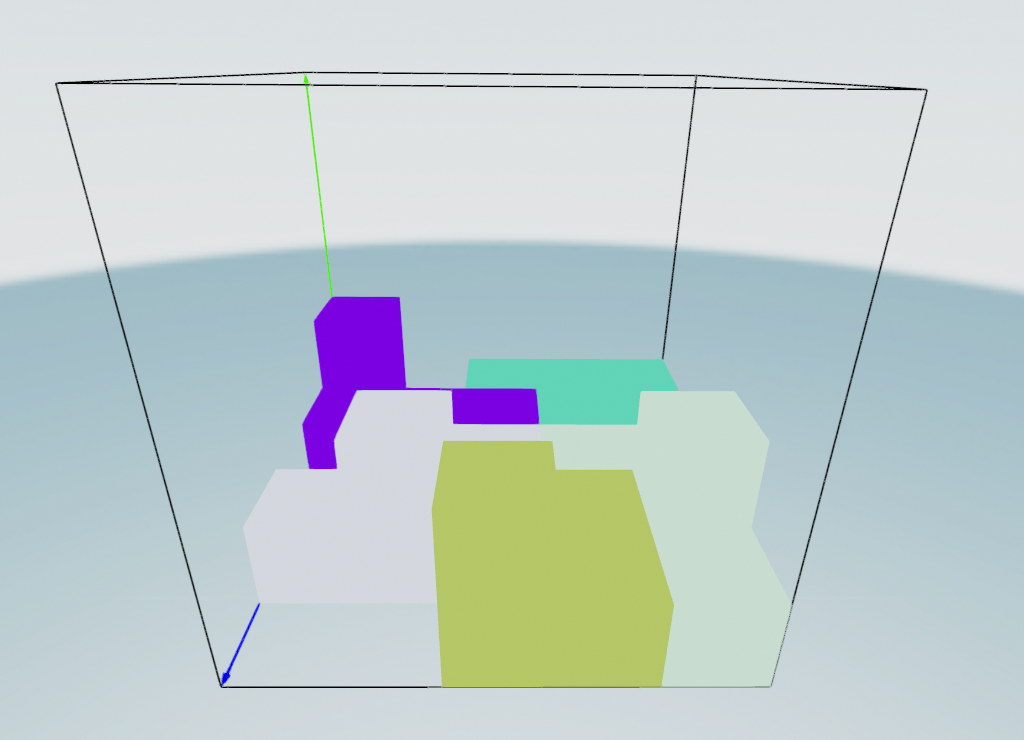
\includegraphics[width=0.95\textwidth]{images/hape.png}
        \caption{HAPE.}
        \label{fig:hape}
    \end{subfigure}
    \hfill
    \begin{subfigure}[b]{0.3\textwidth}
        \centering
        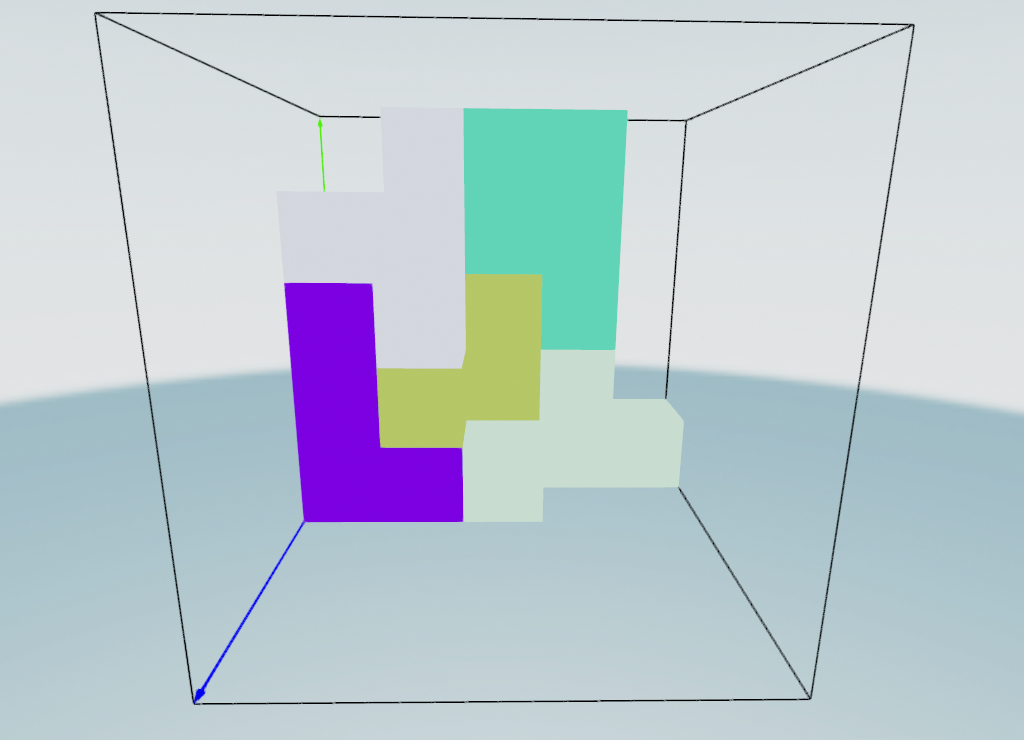
\includegraphics[width=0.95\textwidth]{images/hm.png}
        \caption{Heightmap Minimization (HM).}
        \label{fig:hm}
    \end{subfigure}
       \caption{Five randomly generated polycubes packed in a\\container using different heuristics.}
       \label{fig:polycubes}
\end{figure}

A significant challenge for BPP with irregular shapes is that a single shape can have infinitely many orientations, leading to an infinite number of possible placements in the container.
For this reason, the problem is often simplified by discretizing the possible orientations of the shapes \cite{Zhao2022general}.
In the case of polycubes, each polycube can have up to 24 unique orientations \cite{Ronan2006}.
Although a significant increase compared to the six possible orientations of a regular cuboid, this is still manageable without needing any additional discretization.
This places the complexity of the online polycube packing problem somewhere between regular and irregular shapes, making it an interesting problem to study.

Due to the limited information available, problems in an online setting cannot be solved using traditional search-based methods \cite{Zhao2022pct}.
Online BPP is usually solved using heuristics, but more recently learning-based approaches like deep reinforcement learning (DRL) have been shown to perform better under certain conditions \cite{Zhao2022pct}.
DRL is a combination of deep learning and reinforcement learning: a branch of machine learning in which an agent learns a policy from interacting with an environment \cite{Mousavi2018}.
For more complex variants of online BPP, like irregular shapes, the action space can be too large for DRL to find a good policy \cite{Zhao2022pct}.
However, it has been shown that DRL can still be effective for these problems when restricting the action space using heuristics \cite{Zhao2022pct}\cite{Zhao2022general}.

The main goal of this thesis is to investigate the performance of DRL in solving the online polycube packing problem.
We aim to answer the following research questions:

\begin{enumerate}
    \item Can online polycube packing be solved using deep reinforcement learning?
    \item How does the performance of deep reinforcement learning compare to traditional heuristics?
    \item Can the performance of deep reinforcement learning be improved by using heuristics to restrict the action space?
\end{enumerate}

The remainder of this thesis is structured as follows:
Section \ref{sec:methods} describes the methods used for our research, while Section \ref{sec:implementation} provides details on our exact implementation for reproducibility.
In Section \ref{sec:experiments}, we present the experiments conducted to answer our research questions, and in Section \ref{sec:results}, we present the results.
Finally, in Section \ref{sec:discussion}, we discuss the implications of our findings, and we conclude the thesis in Section \ref{sec:conclusion}.

%
% METHODS
%
\section{Methods} \label{sec:methods}
In this section we describe the methods used for our research.

\subsection{Heuristics} \label{sec:methods:heuristics}
Since online problems cannot be solved using traditional search-based methods, many heuristics have been proposed instead \cite{Zhao2022pct}.
This means that we have a vast pool of heuristics to choose from for our research.
We decided on choosing three heuristics that have been shown to perform well on online packing problems:

\subsubsection{Bottom-Left-Back-Fill}
Bottom-Left-Back-Fill (BLBF) is a simple heuristic that tries to pack items as much to the bottom, left, and back of the container as possible (see Figure \ref{fig:blbf}).
Although this sounds quite arbitrary, it actually resembles the way humans tend to pack items in real life \cite{Zhao2022general} \cite{Karabulut2005}.
It has been a favorite for packing problems for a long time due to its simplicity and good performance with regular shapes \cite{Zhao2022pct}.

\subsubsection{HAPE}
Heuristic Algorithm based on the principle of minimum total Potential Energy, commonly called HAPE, was one of the first heuristics used for efficiently packing irregular shapes \cite{Zhao2022general} \cite{Xiao2011}.
It works by calculating the total potential energy of the items in the container, and placing items in a way that minimizes this value (see Figure \ref{fig:hape}).
In practice, this means that items are placed in a way that keeps the center of mass of the container as low as possible \cite{Zhao2022general} \cite{Xiao2011}.

\subsubsection{Heightmap Minimization}
Lastly, Heightmap Minimization (HM) is a slightly more complex heuristic that is currently seen as one of the best performing heuristics for packing irregular shapes \cite{Zhao2022general}.
It works by flattening the container into a 2D grid, as if it is observing the container through a camera positioned above, and placing items in a way that minimizes the total occupied area as seen from this perspective (see Figure \ref{fig:hm}) \cite{Wang2018}.
This results in a more vertical packing, which is less intuitive, but has been shown to perform well for similar online packing problems \cite{Zhao2022general}.

\subsection{Deep Reinforcement Learning}

\subsubsection{Markov Decision Process}
To solve the online polycube packing problem using deep reinforcement learning, we first need to define the problem as a Markov Decision Process (MDP).
An MDP is a tuple $(\mathbf{S}, \mathbf{A}, \mathbf{P}, \mathbf{R})$, where $\mathbf{S}$ is the set of states, $\mathbf{A}$ is the set of actions, $\mathbf{P}$ is the transition probability function, and $\mathbf{R}$ is the reward function \cite{Sutton1998}.

The state $s_t \in \mathbf{S}$ at time step $t$ is defined as the tuple $s_t = (C_t, p_t)$, where $C_t$ is the current state of the container and $p_t$ is the next polycube to be packed at this time step \cite{Zhao2022pct}.

The action $a_t \in \mathbf{A}$ at time step $t$ is defined as the tuple $a_t = (r, x, y, z)$, where $r$ is the orientation of the polycube and $(x, y, z)$ is the position of the polycube in the container.

The transition probability function $\mathbf{P}(s_{t + 1} | s_t)$ is fully stochastic, as the next polycube to be packed is uniformly sampled from the set of all possible polycubes when we move to the next time step.

For the reward function $\mathbf{R}(s_t, a_t)$ there is no real consensus when it comes to online packing problems.
Since our end goal is to pack as many polycubes as possible, we define the reward function to be the number of polycubes packed at the end of the episode:

\begin{equation}
    \mathbf{R}(s_t, a_t) =
    \begin{cases}
        t & \text{if } s_t \text{ is terminal} \\
        0 & \text{otherwise}
    \end{cases}
    \label{eq:reward_function}
\end{equation}

\subsubsection{Action Masking}
When looking at the action space described above, we can see that the number of possible actions can easily become too large to efficiently learn a policy.
Even a small container of size $4 \times 4 \times 4$ with 24 orientations per polycube results in an action space of size $4 \times 4 \times 4 \times 24 = 1536$.
While still theoretically learnable, the situation is worsened by the fact that most of these actions will be invalid due to collisions with other polycubes.
To solve this issue, we "mask out" invalid actions and sample solely from the remaining valid actions, a technique known as invalid action masking \cite{Huang2020}.

To further reduce the size of the action space, we can also use heuristics to restrict the action space to only the most promising actions. This technique is known as heuristic action masking, and is commonly used when packing irregular shapes with an even larger action space \cite{Zhao2022general}.
During our experiments, we will compare the performance of the DRL agent with and without heuristic action masking.

\subsubsection{Proximal Policy Optimization}
Since we are dealing with a large state and action space in a stochastic environment, we restrict our choice of DRL algorithm to on-policy, model-free algorithms that work with function approximation.
One of the most popular algorithms in this category is Proximal Policy Optimization (PPO).
PPO is a policy gradient method that aims to maximize the expected return by iteratively sampling data from the environment and updating an objective function using stochastic gradient ascent \cite{Schulman2017}.
PPO outperforms most other policy gradient methods in a range of environments, and is known for its balance between sample efficiency, complexity, and ease of use \cite{Schulman2017}.
Since the introduction of PPO in 2017, many variations have been proposed, but these often come with small improvements at the cost of increased complexity, which is why we decided on using the original PPO algorithm for our research.

%
% IMPLEMENTATION
%
\section{Implementation} \label{sec:implementation}
In this section, we will provide the exact details of our implementation.
All code was written in Python 3.9.13, together with Gymnasium 0.29.1, Stable-Baselines3 2.3.0, sb3-contrib 2.3.0, and TensorFlow 2.16.1 \cite{gymnasium} \cite{stable-baselines3} \cite{tensorflow}.

\subsection{Packing Environment}
We define the container as a tensor of size $(X, Y, Z)$, where $X$, $Y$, and $Z$ are the dimensions of the container.
Each element in the tensor represents a unit cube, so naturally adding a polycube to the container will change the value of multiple elements in the tensor.
The polycubes are represented as (smaller) tensors, where each non-zero element represents a unit cube in the polycube.
When we successfully add a polycube to the container, the next polycube to be packed is uniformly sampled from the set of all possible polycubes inside a given size range.
For example, when the size range is $[3, 5]$, all polycubes of size $3$, $4$, and $5$ are added to the set where the next polycube is sampled from.

To check if a polycube can be added to the container at a given position and orientation, we first check if the polycube fits inside the container, and then check if the polycube collides with any other polycube already in the container.
This last step is done by creating a mask of the polycube at the given orientation and applying it to the container at the given position.
If applying this mask results in any collisions, the polycube cannot be added to the container at this position and orientation.
To compute all feasible positions for a polycube in a container, we use the algorithm described in Algorithm \ref{alg:feasible_positions}.
Note that calls to this algorithm are optimized using a cache, as iterating over all positions and orientations is very computationally expensive.

\begin{algorithm}[!htb]
    \caption{Feasible Positions}\label{alg:feasible_positions}
    \begin{algorithmic}[1]
    \State \textbf{given} $C$, $p$ \Comment{container and polycube}
    \State feasible\_positions = []
    \For{$(x, y, z)$ in $C$}
        \For{$r$ in $p$.orientations()}
            \If{$C$.fit($p$, $r$, $x$, $y$, $z$)}
                \State feasible\_positions.append($r$, $x$, $y$, $z$)
            \EndIf
        \EndFor
    \EndFor
    \end{algorithmic}
\end{algorithm}

\subsection{Heuristics} \label{sec:implementation:heuristics}
All heuristics were implemented as functions that take in the current state of the container, and return a normalized score in range $[0, 1]$ for how "good" the current state is.

\subsubsection{Bottom-Left-Back-Fill}
We compute the center of mass of the container by averaging the coordinates of all unit cubes in the container.
To determine how much to the bottom, left, and back the container is currently packed we use the following formula:

\begin{equation}
    1 - \frac{|CoM|}{\left\lvert\begin{pmatrix}
        X \\
        Y \\
        Z
    \end{pmatrix} - \begin{pmatrix}
        1 \\
        1 \\
        1
    \end{pmatrix}\right\rvert }
    \label{eq:blbf}
\end{equation}

Here $CoM$ is the center of mass of the container and $(X, Y, Z)$ are the dimensions of the container.

\subsubsection{HAPE}
Similarly to BLBF, we compute the center of mass of the container by averaging the coordinates of all unit cubes in the container.
To determine how low the center of mass is we use the following formula:

\begin{equation}
    \frac{Y - CoM}{Y}
    \label{eq:hape}
\end{equation}

Here $CoM$ is the center of mass of the container and $Y$ is the height of the container.

\subsubsection{Heightmap Minimization}
To compute the score for the heightmap minimization heuristic we first flatten the container into a 2D matrix, and then calculate the occupied area of this matrix as a percentage of the total area.
As the goal is to minimize the occupied area, we use the inverse of this value as the score.

\subsection{Agents}
All agents follow a standard template, where given a state $s_t$ (the current container and the next polycube to be packed), they return an action $a_t$ (the position and orientation of the polycube in the container).

\subsubsection{Greedy Agent}
The greedy agent uses the heuristics described in Sections \ref{sec:methods:heuristics} and \ref{sec:implementation:heuristics} to determine the best position and orientation for the next polycube to be packed.
The agent is initialized with a list of heuristics, and uses the algorithm described in Algorithm \ref{alg:greedy} to determine the best action.

\begin{algorithm}[!htb]
    \caption{Greedy Agent}\label{alg:greedy}
    \begin{algorithmic}[1]
    \State \textbf{given} $C$, $p$, $H$ \Comment{container, polycube, heuristics}
    \State \textbf{given} feasible\_positions
    \State scores = []
    \For{heuristic in $H$}
        \For{position in feasible\_positions}
            \State $C^\prime$ = $C$.add($p$, position)
            \State scores[heuristic, position] = heuristic($C^\prime$)
        \EndFor
    \EndFor
    \State scores = mean(scores) \Comment{average scores over position}
    \State best\_position = argmax(scores)
    \end{algorithmic}
\end{algorithm}

\subsubsection{PPO Agent} \label{sec:implementation:ppo}
The PPO agent is based on the "Maskable PPO" implementation provided by the \textit{sb3-contrib} package \cite{stable-baselines3}.
The agent uses the current state together with an action mask to determine the best action to take.
When not using heuristics to restrict the actions space, this action mask is equal to the feasible positions as computed in Algorithm \ref{alg:feasible_positions}.
When using heuristics to restrict the action space, the action mask is created using the algorithm described in Algorithm \ref{alg:heuristic_mask}, where $n$ is a hyperparameter that determines how many of the best actions are kept.
Note that in order to feed states with a variable polycube size to the policy network, the polycube is first padded to the size of the container.

\begin{algorithm}[!htb]
    \caption{Heuristic Action Mask}\label{alg:heuristic_mask}
    \begin{algorithmic}[1]
    \State \textbf{given} $C$, $p$, $H$ \Comment{container, polycube, heuristics}
    \State \textbf{given} feasible\_positions
    \State scores = []
    \For{heuristic in $H$}
        \For{position in feasible\_positions}
            \State $C^\prime$ = $C$.add($p$, position)
            \State scores[heuristic, position] = heuristic($C^\prime$)
        \EndFor
    \EndFor
    \State scores = mean(scores) \Comment{average scores over position}
    \State best\_actions = scores.sort().head($n$) \Comment{$n$ best actions}
    \State mask = zeros(action\_space)
    \State mask[best\_actions] = 1
    \end{algorithmic}
\end{algorithm}

%
% EXPERIMENTS
%
\section{Experiments} \label{sec:experiments}
In order to answer our research questions, we conducted a series of experiments related to the performance of our agents.
In total, three agents were trained per container size: a PPO agent with default hyperparameters (PPO-D), a PPO agent with optimized hyperparameters (PPO-O), and a PPO agent with optimized hyperparameters and heuristic action masking (PPO-H).
The exact hyperparameters used for the training, along with the hyperparameter tuning process, can be found in Appendix \ref{app:hyperparameters}.
As training the agents is computationally expensive, we only performed experiments on four different container sizes: $3 \times 3 \times 3$, $5 \times 3 \times 3$, $4 \times 4 \times 4$, and $6 \times 4 \times 4$.
As a baseline, we compared the performance of our agents to a greedy agent that uses a combination of the Bottom-Left-Back-Fill and Heightmap Minimization heuristics for the $3 \times 3 \times 3$ container, and a combination of the Bottom-Left-Back-Fill and HAPE heuristics for all other containers.
This combination of heuristics was chosen because it performed best in our preliminary experiments, which can be found in Appendix \ref{app:heuristics}.
Note that all experiments were run on a laptop with a 2.6 GHz Intel Core i7-9750H processor, 16 GB of RAM, and an NVIDIA GeForce GTX 1650 GPU, unless stated otherwise.

\subsection{Training Procedure}
To train the agents, we used the training framework provided by the \textit{Gymnasium} and \textit{Stable-Baselines3} packages \cite{gymnasium} \cite{stable-baselines3}.
During training, the agents are trained on a single container size for a fixed number of steps, where each step corresponds to a single polycube being packed.
The network weights are updated at the end of every epoch, which is defined as a smaller number of steps depending on the container size (see Appendix \ref{app:hyperparameters}).
All agents were trained until convergence, which was determined by monitoring the mean reward and the entropy loss, sampled every epoch.
The mean reward tells us how well the agent is performing, while the entropy loss tells us how the agent is balancing exploration with exploitation (a higher entropy loss equals more exploitation).

\subsection{Evaluation}
To evaluate the performance of the agents, we ran the trained agents and the greedy agents on 10,000 randomly generated polycube sequences for each container size.
To limit the influence of the randomness of the environment as much as possible, all agents were tested on the same polycube sequences.
The upper bound of the polycube size was set to the largest dimension of the container, while the lower bound was set to $3$ (for example, the $5 \times 3 \times 3$ container will be packed with a mix of polycubes of size $3$, $4$ and $5$).
The performance of the agents was measured in terms of the number of polycubes packed and the mean time it took to pack a single polycube.
The mean time taken to pack a single polycube was measured as the time between the environment being reset and the environment returning a terminal state, divided by the number of polycubes packed.

%
% RESULTS
%
\section{Results} \label{sec:results}
In this section we present the results of our experiments.

\subsection{Training} \label{sec:results:training}
In Figures \ref{fig:3x3x3-reward}, \ref{fig:3x3x3-entropy}, \ref{fig:5x3x3-reward}, \ref{fig:5x3x3-entropy}, \ref{fig:4x4x4-reward}, \ref{fig:4x4x4-entropy}, \ref{fig:6x4x4-reward}, and \ref{fig:6x4x4-entropy} the mean reward and entropy loss over time of different PPO configurations on the various container sizes can be seen.

\begin{figure}
    \centering
    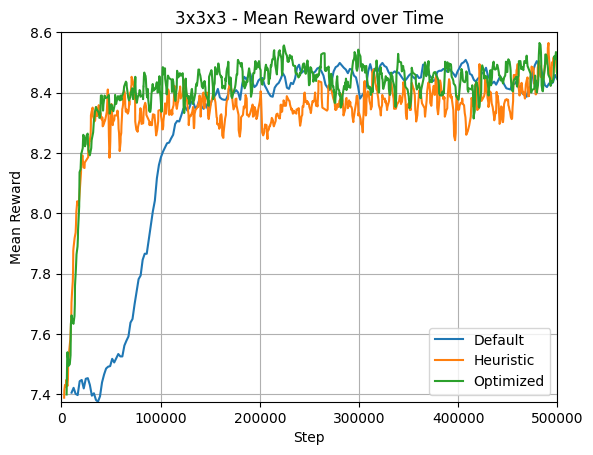
\includegraphics[scale=0.525]{images/3x3x3-reward.png}
    \caption{Mean reward over time of different PPO configurations on a $3 \times 3 \times 3$ container.\label{fig:3x3x3-reward}}
\end{figure}

\begin{figure}
    \centering
    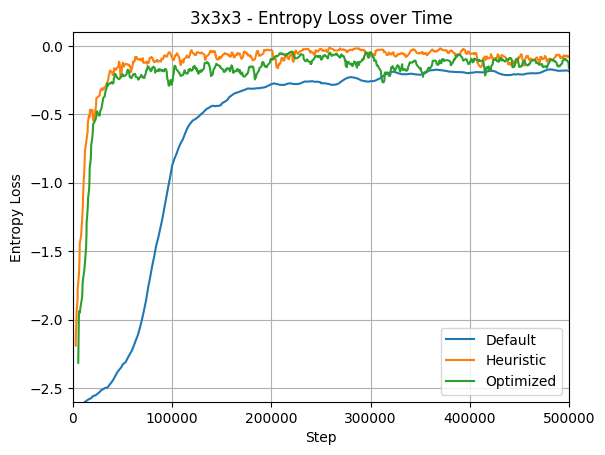
\includegraphics[scale=0.525]{images/3x3x3-entropy.png}
    \caption{Entropy loss over time of different PPO configurations on a $3 \times 3 \times 3$ container.\label{fig:3x3x3-entropy}}
\end{figure}

\begin{figure}
    \centering
    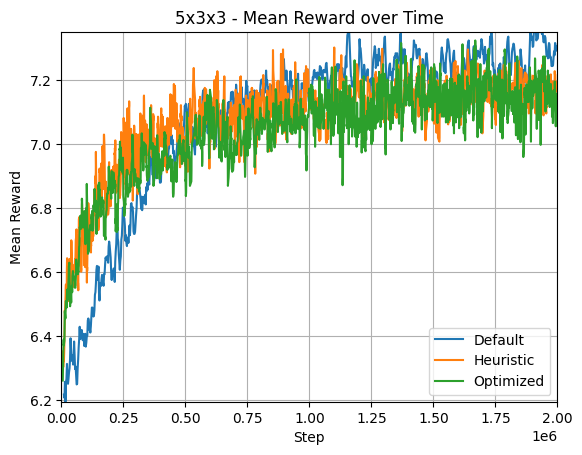
\includegraphics[scale=0.525]{images/5x3x3-reward.png}
    \caption{Mean reward over time of different PPO configurations on a $5 \times 3 \times 3$ container.\label{fig:5x3x3-reward}}
\end{figure}

\begin{figure}
    \centering
    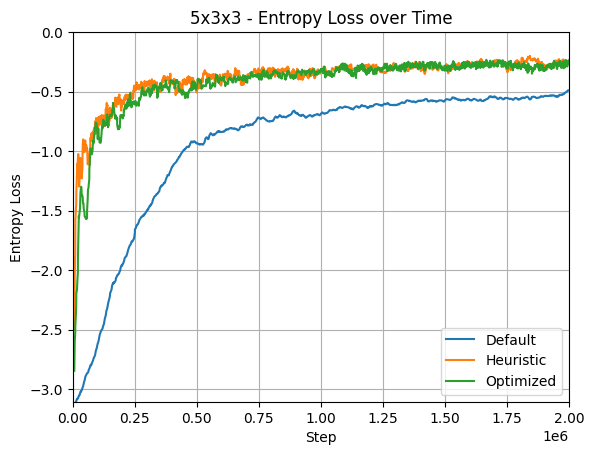
\includegraphics[scale=0.525]{images/5x3x3-entropy.png}
    \caption{Entropy loss over time of different PPO configurations on a $5 \times 3 \times 3$ container.\label{fig:5x3x3-entropy}}
\end{figure}

\begin{figure}
    \centering
    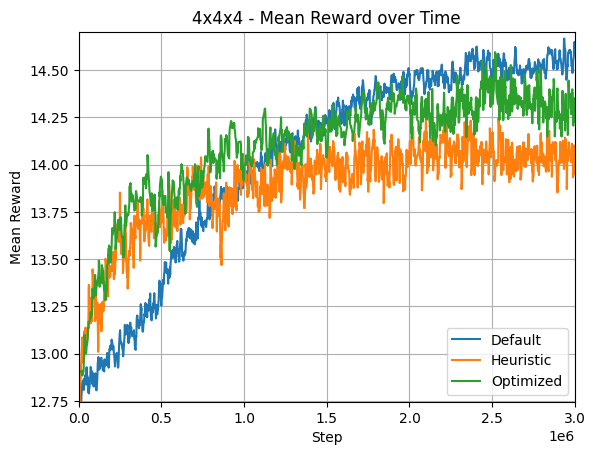
\includegraphics[scale=0.525]{images/4x4x4-reward.png}
    \caption{Mean reward over time of different PPO configurations on a $4 \times 4 \times 4$ container.\label{fig:4x4x4-reward}}
\end{figure}

\begin{figure}
    \centering
    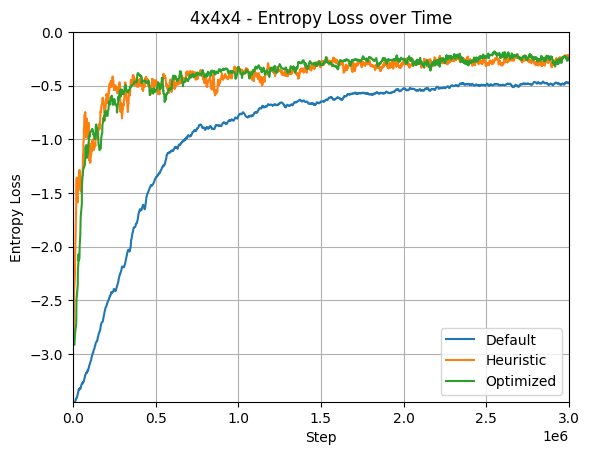
\includegraphics[scale=0.525]{images/4x4x4-entropy.png}
    \caption{Entropy loss over time of different PPO configurations on a $4 \times 4 \times 4$ container.\label{fig:4x4x4-entropy}}
\end{figure}

\newpage
\begin{figure}
    \centering
    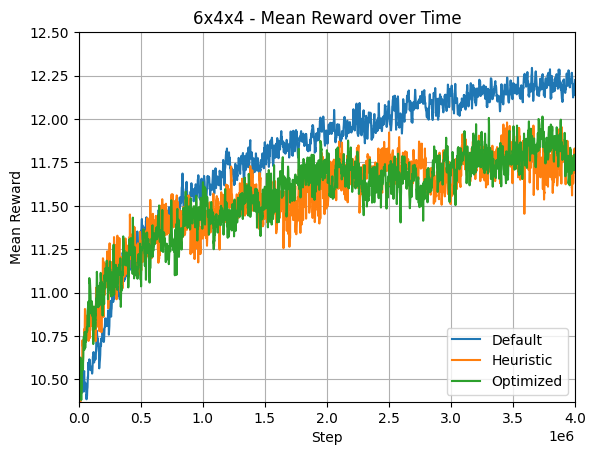
\includegraphics[scale=0.525]{images/6x4x4-reward.png}
    \caption{Mean reward over time of different PPO configurations on a $6 \times 4 \times 4$ container.\label{fig:6x4x4-reward}}
\end{figure}

\begin{figure}
    \centering
    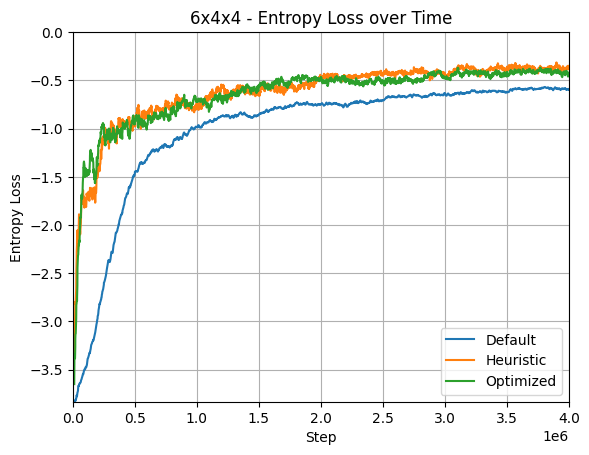
\includegraphics[scale=0.525]{images/6x4x4-entropy.png}
    \caption{Entropy loss over time of different PPO configurations on a $6 \times 4 \times 4$ container.\label{fig:6x4x4-entropy}}
\end{figure}

In these figures, the PPO agent with default hyperparameters (PPO-D) is shown in blue, the optimized PPO agent with heuristic action masking (PPO-H) is shown in orange, and the optimized PPO agent without heuristic action masking (PPO-O) is shown in green.
The graphs are created by sampling the mean reward and entropy loss every epoch, and then averaging these values using a moving average with a window size of five.
The total wall time for training the different PPO configurations on the different container sizes can be found in Table \ref{tab:training-time}.

\begin{table}[!htb]
    \centering
    \caption{Wall time for training different PPO configurations on different container sizes. Times marked with an asterisk ($^\ast$) were trained on an Intel Core i7-7800X processor, 32 GB of RAM, and an NVIDIA GeForce RTX 4060 GPU.\label{tab:training-time}}
    \begin{tabular}{l|c|c|c}
     & \textbf{Default} & \textbf{Heuristics} & \textbf{Optimized} \\ \hline
    $3 \times 3 \times 3$ & 1.5 hr & 2 hr & 1.5 hr \\
    $5 \times 3 \times 3$ & 8.5 hr & 12 hr & 6.5 hr \\
    $4 \times 4 \times 4$ & 14$^\ast$ hr & 20$^\ast$ hr & 14$^\ast$ hr \\
    $6 \times 4 \times 4$ & 32$^\ast$ hr & 45$^\ast$ hr & 32$^\ast$ hr
    \end{tabular}
\end{table}

\subsection{Evaluation} \label{sec:results:evaluation}
In Figures \ref{fig:3x3x3-pairwise-packed}, \ref{fig:5x3x3-pairwise-packed}, \ref{fig:4x4x4-pairwise-packed}, and \ref{fig:6x4x4-pairwise-packed} the pairwise comparison of the PPO-D, PPO-H, PPO-O, and greedy agents for packing shapes on different container sizes can be seen.

\begin{figure}[!htb]
    \centering
    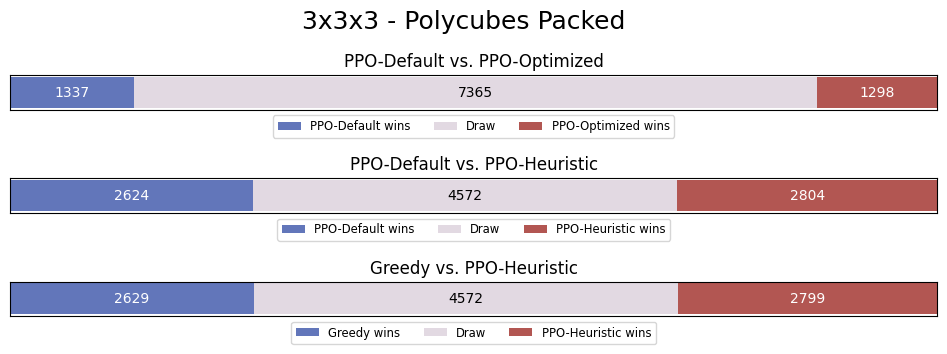
\includegraphics[scale=0.35]{images/3x3x3-pairwise-packed.png}
    \caption{Pairwise comparison of the greedy, PPO-D, PPO-H, and PPO-O agents for packing shapes in a $3 \times 3 \times 3$ container.\label{fig:3x3x3-pairwise-packed}}
\end{figure}

\begin{figure}[!htb]
    \centering
    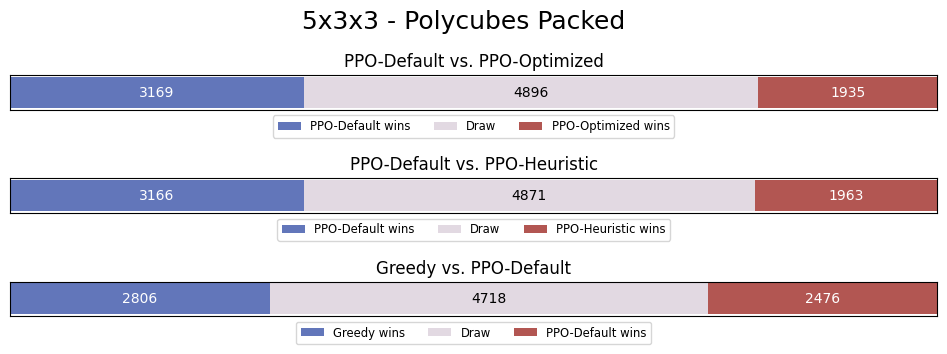
\includegraphics[scale=0.35]{images/5x3x3-pairwise-packed.png}
    \caption{Pairwise comparison of the greedy, PPO-D, PPO-H, and PPO-O agents for packing shapes in a $5 \times 3 \times 3$ container.\label{fig:5x3x3-pairwise-packed}}
\end{figure}

\begin{figure}[!htb]
    \centering
    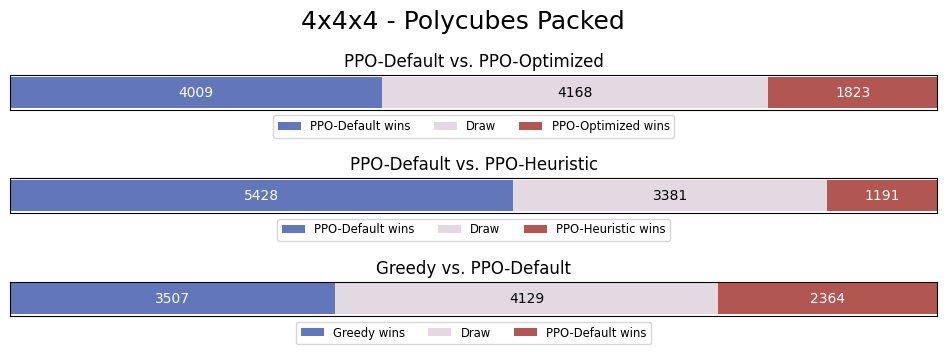
\includegraphics[scale=0.35]{images/4x4x4-pairwise-packed.png}
    \caption{Pairwise comparison of the greedy, PPO-D, PPO-H, and PPO-O agents for packing shapes in a $4 \times 4 \times 4$ container.\label{fig:4x4x4-pairwise-packed}}
\end{figure}

\begin{figure}[!htb]
    \centering
    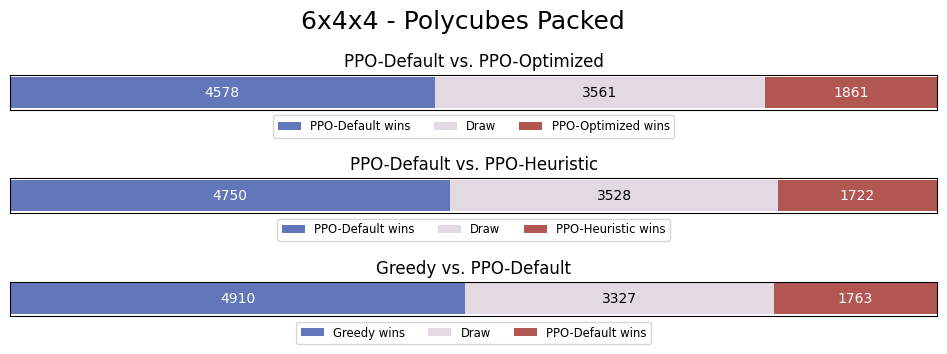
\includegraphics[scale=0.35]{images/6x4x4-pairwise-packed.png}
    \caption{Pairwise comparison of the greedy, PPO-D, PPO-H, and PPO-O agents for packing shapes in a $6 \times 4 \times 4$ container.\label{fig:6x4x4-pairwise-packed}}
\end{figure}

In these figures, the blue bars represent the number of seeds where the first agent packed more polycubes than the second agent, the red bars represent the number of seeds where the second agent packed more polycubes than the first agent, and the gray bars represent the number of seeds where both agents packed the same number of polycubes.
Figure \ref{fig:mean_time_taken} shows the mean wall time to pack a single polycube for all agents on different container sizes, with outliers more than three standard deviations from the mean removed.

\begin{figure}[!htb]
    \centering
    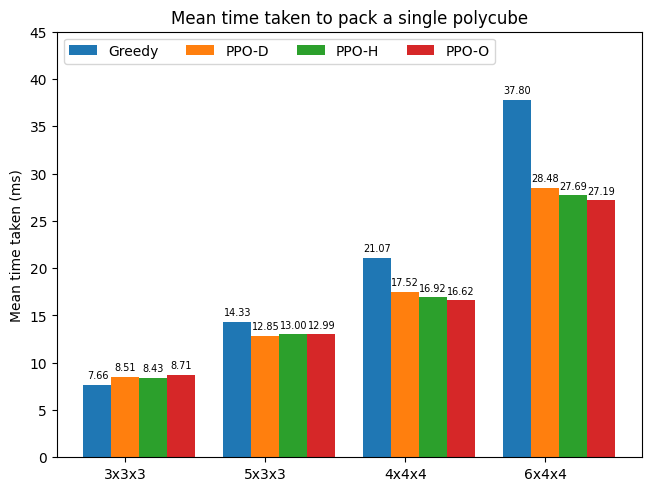
\includegraphics[scale=0.5]{images/mean_time_taken.png}
    \caption{Mean wall time to pack a single polycube for all agents on different container sizes.\label{fig:mean_time_taken}}
\end{figure}

%
% DISCUSSION
%
\section{Discussion} \label{sec:discussion}
Figure \ref{fig:3x3x3-reward} shows that all PPO agents converge to the same mean reward of around 8.5 polycubes packed on the $3 \times 3 \times 3$ container.
Since all polycubes in this container have a size of three, the theoretical maximum number of polycubes that can be packed is nine.
However, the actual maximum number of polycubes that can be packed is dependent on the sequence of polycubes generated by the seed.
There are only two types of polycubes that can be packed in a $3 \times 3 \times 3$ container: a polycube that looks like an 'I' (three cubes placed in a row) and a polycube that looks like an 'L' (two cubes placed in a row with one cube sticking out to the side).
All possible polycubes of size three are just a rotation of one these two polycubes.
Since the packing is online with no prior knowledge of the sequence of polycubes, even a perfect packing algorithm would have to choose whether to leave space for the 'I' polycube or the 'L' polycube at the end of the episode.
This places the average maximum number of polycubes that can be packed in a $3 \times 3 \times 3$ container at around 8.5, even for a perfect packing algorithm.
Since all PPO agents seem to converge towards a mean reward of 8.5, this verifies that the PPO agents are able to successfully solve the online polycube packing problem for the $3 \times 3 \times 3$ container, although there is a noticeable difference in convergence rate between the different configurations.

The results shown in Section \ref{sec:results:training} show that the PPO-H agent consistently converges faster than the PPO-D agent.
This is expected, as heuristic action masking restricts the action space to only the most promising actions.
A more surprising result is that the PPO-O agent seems to match the convergence rate of the PPO-H agent for all container sizes.
This suggests that heuristic action masking might not be as effective as we initially thought, and that the PPO-O agent is able to learn a good policy even without restricting the action space.
This is especially relevant when taking the training time shown in Table \ref{tab:training-time} into account, as the PPO-H agent is significantly slower to train than the other PPO agents.
Heuristic action masking has seen great success in more complex packing problems, like irregular shapes, but our results suggest that the online polycube packing problem at these container sizes is not complex enough for it to outperform other PPO configurations.

Another surprising result is that, despite the slower convergence rate, the PPO-D agent eventually converges to a higher mean reward than the PPO-H and PPO-O agents for all container sizes larger than $3 \times 3 \times 3$.
This suggests that a faster convergence rate does not necessarily lead to a better policy, and that the hyperparameters used for the PPO-O agent are suboptimal for larger container sizes.
Since the hyperparameters of the PPO-O and PPO-H agents were tuned on a $3 \times 3 \times 3$ container, it is possible that these hyperparameters are overfitted to the smaller container size, although we are unable to confirm this without further experiments.

A final interesting result from this section is that the entropy loss of the PPO-D agent seems to be consistently lower than the entropy loss of the other PPO agents.
This suggests that even though the PPO-D agent is able to achieve a higher mean reward than the other PPO agents, it is less "confident" in its policy.
A possible explanation for this would be that the PPO-D agent is able to learn less exploitative policies than the other PPO agents, or that the other PPO agents are too exploitative in their policies, converging too quickly to local optima.
Similar to the difference in convergence rate, further research into the hyperparameters of the PPO-O and PPO-H agents would be needed to confirm this.

The head-to-head results shown in Section \ref{sec:results:evaluation} further confirm that the PPO-D agent is able to outperform the PPO-H and PPO-O agents for all container sizes larger than $3 \times 3 \times 3$.
Using a McNemar's test, we find that the difference in head-to-head performance between the PPO-D and the other PPO agents is statistically significant for all container sizes larger than $3 \times 3 \times 3$ ($p \leq 0.05$).
For the $3 \times 3 \times 3$ container, there is no statistically significant difference in head-to-head performance between the different PPO agents.
This confirms that the PPO-D agent is able to learn a better policy than the PPO-H and PPO-O agents for larger container sizes.

Comparing the performance of the PPO-D agent with the greedy agent, we can see that the greedy agent is able to outperform the PPO-D agent for all container sizes larger than $3 \times 3 \times 3$.
Using a McNemar's test, we find that the difference in head-to-head performance between the PPO-D agent and the greedy agent is statistically significant for all container sizes larger than $3 \times 3 \times 3$ ($p \leq 0.05$).
This confirms that, even though the PPO agents are able to solve the online polycube packing problem, they are not able to match the performance of a greedy agent using a good combination of packing heuristics.

The last metric we evaluated was the mean wall time to pack a single polycube, as shown in Figure \ref{fig:mean_time_taken}.
The results show that all PPO agents are consistently faster than the greedy agent for larger container sizes.
This is expected, as the greedy agent has to iterate over all feasible positions for each polycube, and then calculate the score for each position using its heuristics.
The PPO agents use a policy network that can in theory pack polycubes in a constant time.
In practice this is not the case, as the PPO agents still need to compute the invalid action mask, which requires iterating over every container position.
However, since they skip the step of calculating a heuristic score for every position, they are still consistently faster than the greedy agent for larger container sizes.

%
% CONCLUSION
%
\section{Conclusion} \label{sec:conclusion}
In our research we investigated the performance of deep reinforcement learning agents on the online polycube packing problem.
We aimed to answer the following research questions:

\begin{enumerate}
    \item Can online polycube packing be solved using deep reinforcement learning?
    \item How does the performance of deep reinforcement learning compare to traditional heuristics?
    \item Can the performance of deep reinforcement learning be improved by using heuristics to restrict the action space?
\end{enumerate}

To answer these questions, we trained three different PPO agents on four different container sizes, and compared their performance to a greedy agent using an optimal combination of packing heuristics.
Our results show that the PPO agents are able to solve the online polycube packing problem for all container sizes, but they are not able to match the performance of the greedy agent.
The PPO agents are consistently faster than the greedy agent, but they are on average not able to pack as many polycubes.
The best performing PPO agent is the one with default hyperparameters, which is able to outperform the other PPO agents for all container sizes larger than $3 \times 3 \times 3$.
Heuristic action masking does not seem to improve the performance of the PPO agents, and is significantly slower to train than the other PPO configurations.

Our research is mostly limited by the computational cost of studying this problem.
Hyperparameter tuning, training the agents, and evaluating the agents on different container sizes are all computationally expensive tasks, which limits the number of experiments we can perform.
Future research could try to repeat our experiments on larger container sizes, or with more sophisticated hyperparameter tuning, to see if our results hold.
Especially the hyperparameter tuning could be improved by focusing less on the convergence rate of the agents, and more on the final mean reward on larger container sizes.
Furthermore, the performance of the agents could potentially be improved by using more advanced DRL algorithms, or by changing the state space to include more information about the current state of the container.

%
% REFERENCES
%
\newpage
\bibliographystyle{unsrt}
\bibliography{bibliography}

%
% APPENDIX
%
\newpage
\appendix
\subsection{Hyperparameter Tuning} \label{app:hyperparameters}
The default hyperparameters for PPO, as shown in Table \ref{tab:default-hyperparameters}, were used for training the PPO-D agents.
For other PPO agents, the hyperparameters were tuned using the Optuna framework on a $3 \times 3 \times 3$ container with 100 trails \cite{optuna}.
A $3 \times 3 \times 3$ container was chosen for the hyperparameter tuning because it is the smallest container size, and therefore the fastest to converge.
The hyperparameters that were tuned are the learning rate, the number of steps per epoch, the GAE lambda, the max gradient norm, the entropy coefficient, the value function coefficient, and the clip range.
The exact hyperparameters used for the training of the PPO-H and PPO-O agents can be found in Table \ref{tab:hyperparameters}.

\begin{table}[!htb]
    \centering
    \caption{Default hyperparameters for training PPO agents, as provided  by the \textit{sb3-contrib} package \cite{stable-baselines3}.\label{tab:default-hyperparameters}}
    \begin{tabular}{c|c}
    \textbf{parameter} & \textbf{value} \\ \hline
    learning rate & $0.0003$ \\
    number of steps & $2048$ \\
    batch size & $64$ \\
    update epochs & $10$ \\
    gamma & $0.99$ \\
    GAE lambda & $0.95$ \\
    clip range & $0.2$ \\
    entropy coefficient & $0$ \\
    value function coefficient & $0.5$ \\
    max gradient norm & $0.5$
    \end{tabular}
\end{table}

\begin{table}[!htb]
    \centering
    \caption{Hyperparameters used for training the PPO agents. All hyperparameters not mentioned are kept at their default values as shown in Table \ref{tab:default-hyperparameters}. Values marked with an asterisk ($^\ast$) are scaled based on the size of the container, as shown in Table \ref{tab:scaling}.\label{tab:hyperparameters}}
    \begin{tabular}{c|c}
    \textbf{parameter} & \textbf{value} \\ \hline
    learning rate & $0.0005$ \\
    number of steps & $64 / 128 / 256^\ast$ \\
    entropy coefficient & $0.005$ \\
    heuristics & BLBF + HAPE \\
    $n$ & $50 / 75 / 100 / 200^\ast$
    \end{tabular}
\end{table}

\begin{table}[!htb]
    \centering
    \caption{How the number of steps and $n$ hyperparameters scale based on the size of the container.\label{tab:scaling}}
    \begin{tabular}{c|c|c}
    \textbf{container size} & \textbf{number of steps} & \textbf{n} \\ \hline
    $3 \times 3 \times 3$ & $64$ & $50$ \\
    $5 \times 3 \times 3$ & $128$ & $75$ \\
    $4 \times 4 \times 4$ & $128$ & $100$ \\
    $6 \times 4 \times 4$ & $256$ & $200$
    \end{tabular}
\end{table}

For PPO agents with heuristic action masking, the BLBF and HAPE heuristics were used to create the action mask.
This combination was chosen because it performed best in our preliminary experiments, as shown in Appendix \ref{app:heuristics}.
The hyperparameter $n$, as described in Section \ref{sec:implementation:ppo}, was also tuned using the Optuna framework. 
Both the number of steps and the hyperparameter $n$ are scaled based on the size of the container, as shown in Table \ref{tab:scaling}.

\subsection{Heuristic Experiments} \label{app:heuristics}
In order to determine the best combination of heuristics for the greedy agent, we conducted a series of experiments on all possible combinations of the Bottom-Left-Back-Fill, HAPE, and Heightmap Minimization heuristics.
Throughout these experiments we refer to the different combinations as shown in Table \ref{tab:heuristics}.
Here BLBF stands for Bottom-Left-Back-Fill, HM stands for Heightmap Minimization along the vertical axis, and HM+ stands for Heightmap Minimization along all axes.

\begin{table}[!htb]
    \centering
    \caption{Heuristic combinations used in preliminary experiments.\label{tab:heuristics}}
    \begin{tabular}{c|c}
    \textbf{agent no.} & \textbf{heuristics} \\ \hline
    1 & BLBF \\
    2 & HAPE \\
    3 & HM \\
    4 & HM+ \\
    5 & BLBF, HAPE \\
    6 & BLBF, HM \\
    7 & BLBF, HM+ \\
    8 & HAPE, HM \\
    9 & HAPE, HM+ \\
    10 & BLBF, HAPE, HM \\
    11 & BLBF, HAPE, HM+
    \end{tabular}
\end{table}

To evaluate the performance of the different heuristic combinations, we ran each combination on 100 randomly generated polycube sequences for each container size, and measured the number of polycubes packed and the time it took to pack them.
The results of these experiments can be found in Figures \ref{fig:heuristic-experiments-3x3x3}, \ref{fig:heuristic-experiments-5x3x3}, \ref{fig:heuristic-experiments-4x4x4}, and \ref{fig:heuristic-experiments-6x4x4}.
In the top half of the figure the mean number of polycubes packed can be seen, while in the bottom half the mean time it took to pack a single polycube can be seen in milliseconds.

The results show that the combination of BLBF and HM (agent 6), as well as the combination of BLBF, HAPE and HM+ (agent 11) perform best for the $3 \times 3 \times 3$ container.
Since the combination of BLBF and HM has a lower average time per polycube, we chose this combination as the baseline for the $3 \times 3 \times 3$ container.
For the other containers, the combination of BLBF and HAPE (agent 5) consistently performs best.

\begin{figure}[!htb]
    \centering
    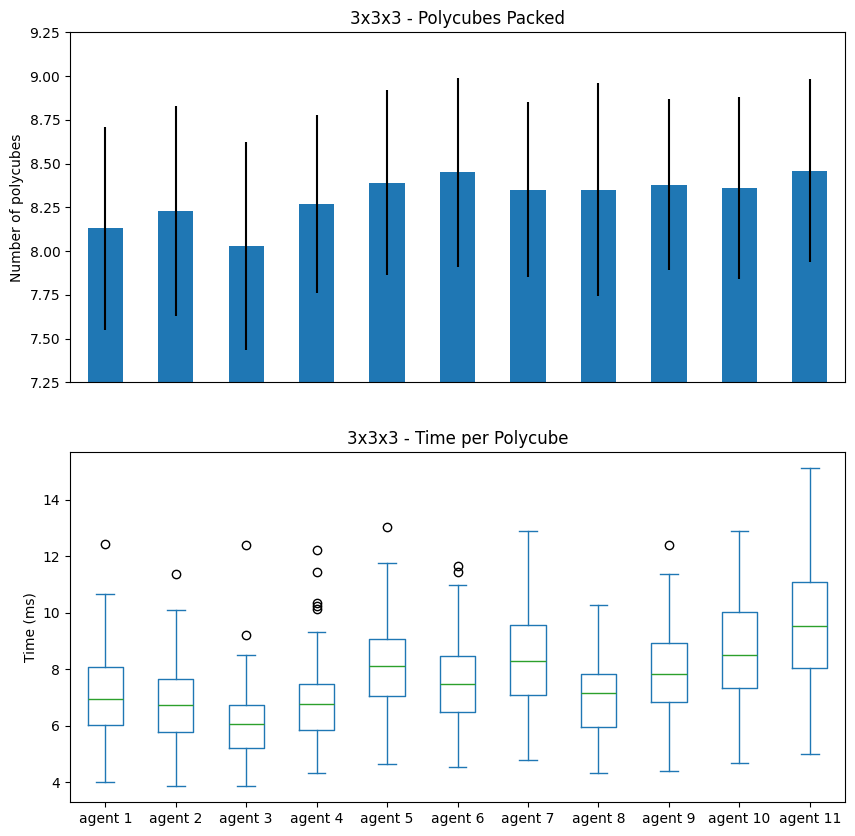
\includegraphics[scale=0.4]{images/heuristic-experiments-3x3x3.png}
    \caption{Performance of different heuristic combinations on a $3 \times 3 \times 3$ container.\label{fig:heuristic-experiments-3x3x3}}
\end{figure}

\begin{figure}[!htb]
    \centering
    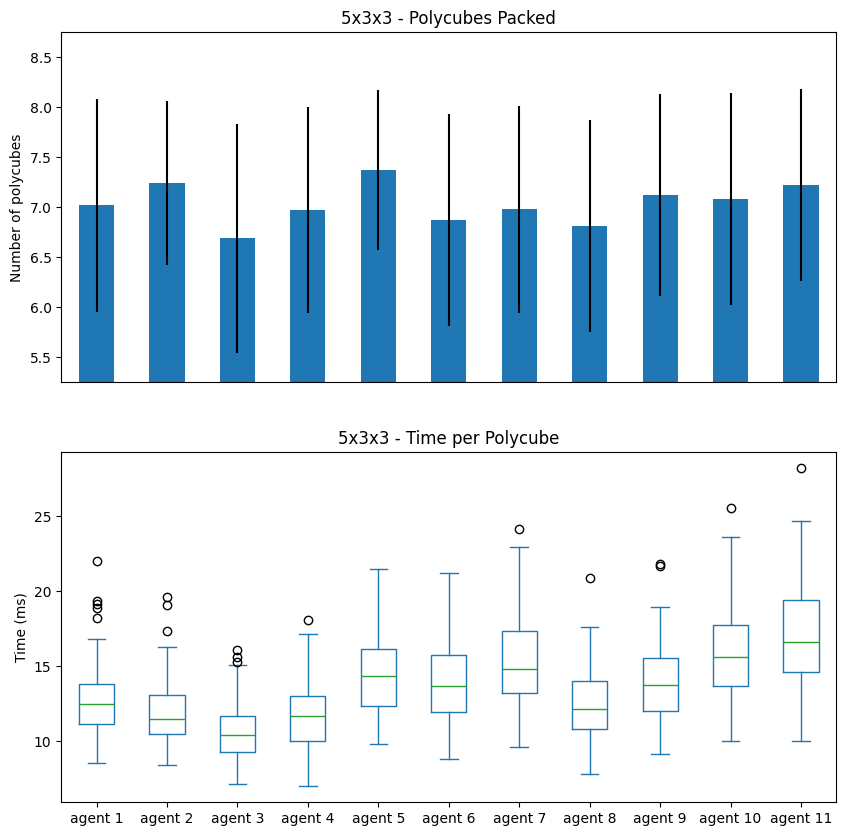
\includegraphics[scale=0.4]{images/heuristic-experiments-5x3x3.png}
    \caption{Performance of different heuristic combinations on a $5 \times 3 \times 3$ container.\label{fig:heuristic-experiments-5x3x3}}
\end{figure}

\begin{figure}[!htb]
    \centering
    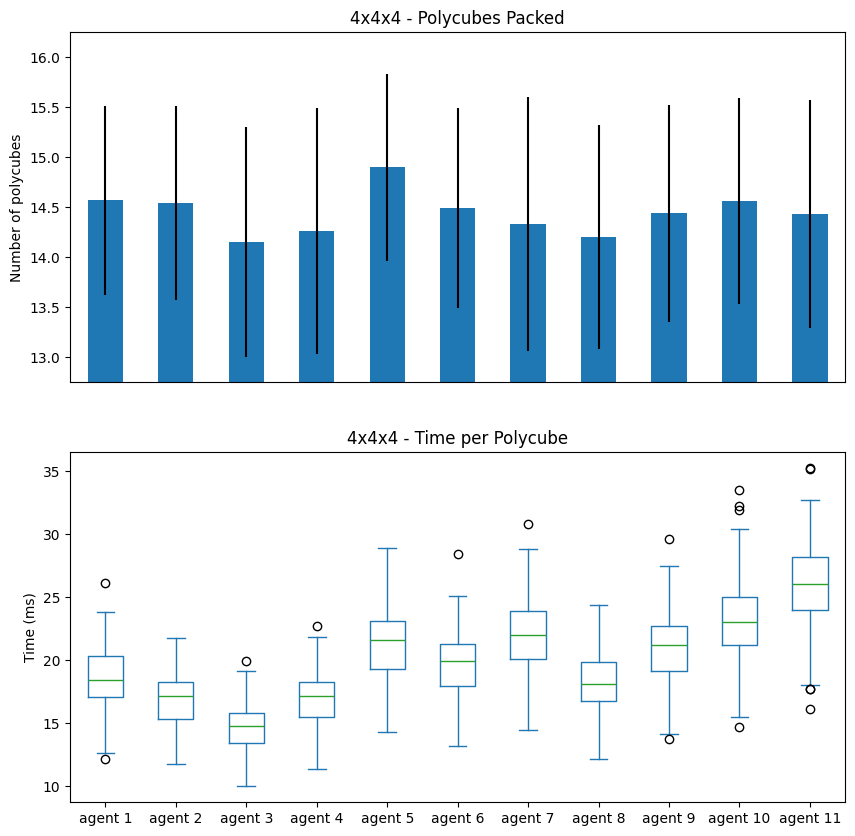
\includegraphics[scale=0.4]{images/heuristic-experiments-4x4x4.png}
    \caption{Performance of different heuristic combinations on a $4 \times 4 \times 4$ container.\label{fig:heuristic-experiments-4x4x4}}
\end{figure}

\begin{figure}[!htb]
    \centering
    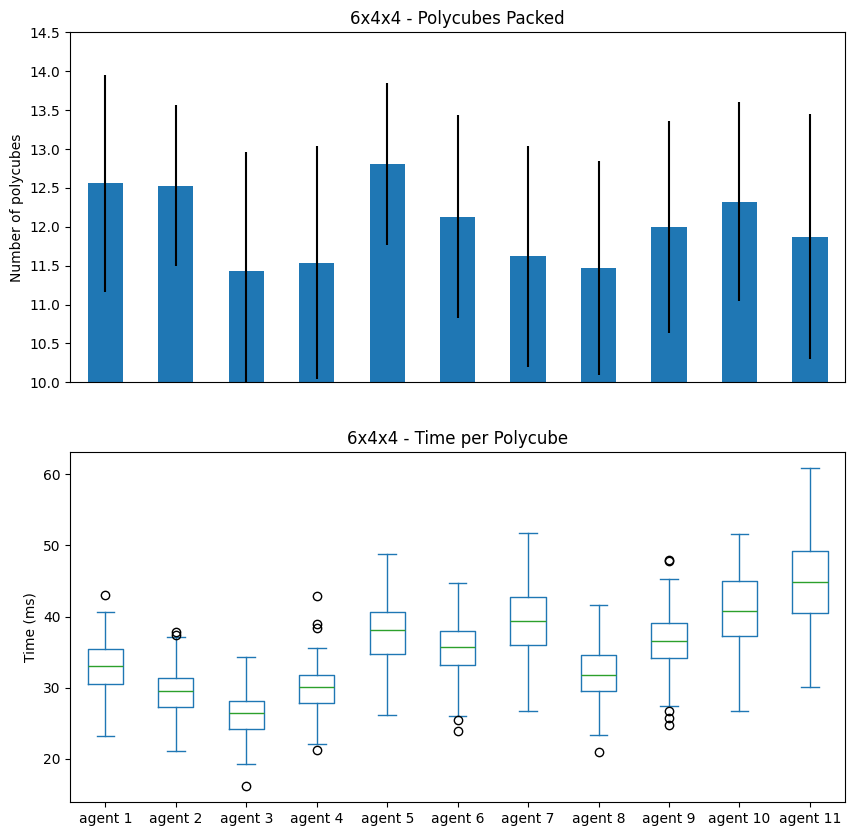
\includegraphics[scale=0.4]{images/heuristic-experiments-6x4x4.png}
    \caption{Performance of different heuristic combinations on a $6 \times 4 \times 4$ container.\label{fig:heuristic-experiments-6x4x4}}
\end{figure}

\subsection{Visualized Results} \label{app:visualized_results}
In this section we provide a few reference images to help visualize the packing of polycubes in different container sizes.
The images show the result of running all agents on a fixed container size with a specific seed, thus packing the same polycube sequence.
In these images, the algorithm name is shown under the packed container, with the number of polycubes it was able to pack in brackets.
The images are shown in Figures \ref{fig:vis-3x3x3-99}, \ref{fig:vis-5x3x3-42}, \ref{fig:vis-4x4x4-42}, \ref{fig:vis-6x4x4-42}, and \ref{fig:vis-6x4x4-99}.

\newpage
\onecolumn
\begin{figure}[!htb]
    \centering
    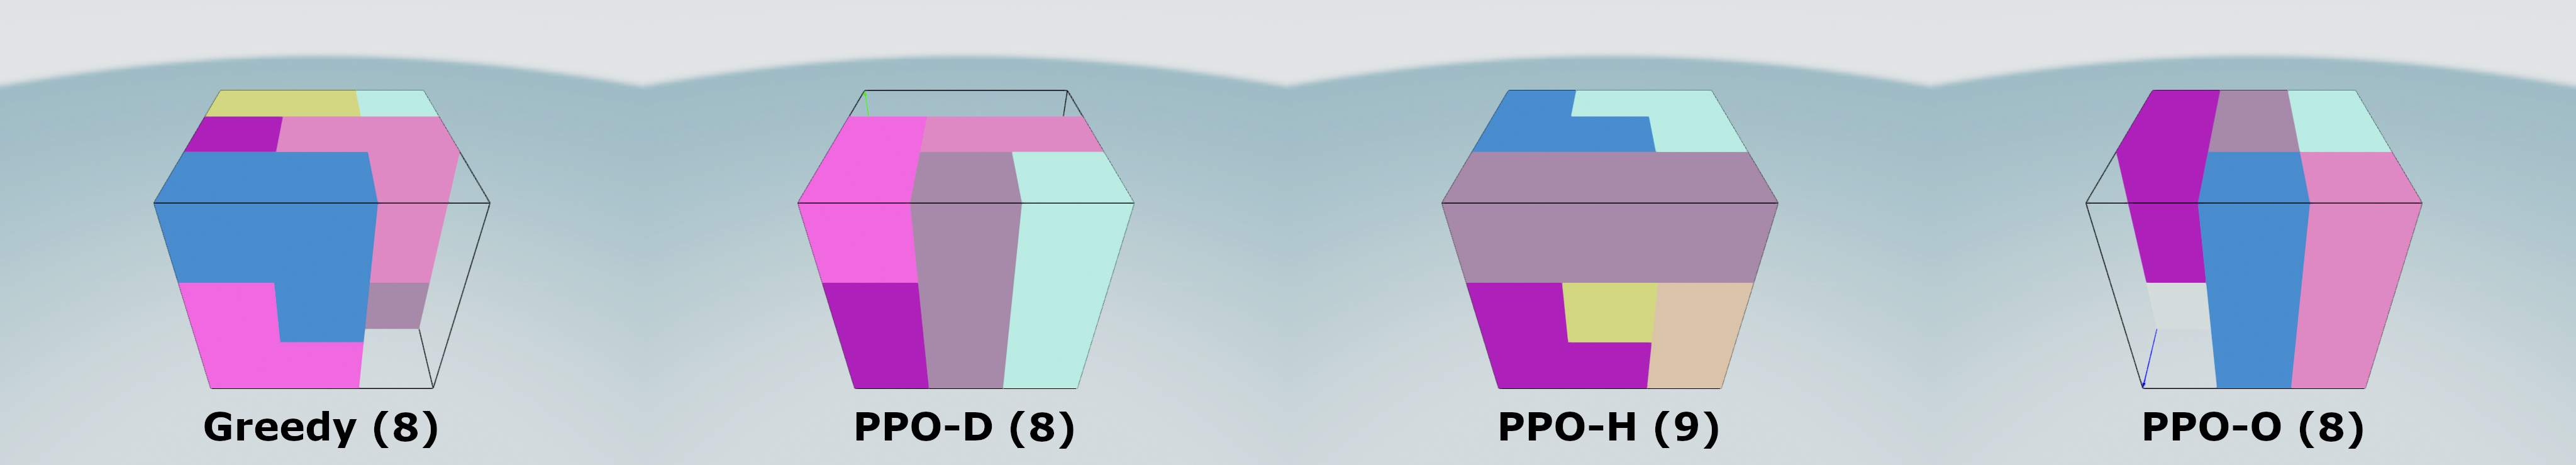
\includegraphics[scale=0.125]{images/vis-3x3x3-99.png}
    \caption{Packing on a $3 \times 3 \times 3$ container with a seed of 99.\label{fig:vis-3x3x3-99}}
\end{figure}

\begin{figure}[!htb]
    \centering
    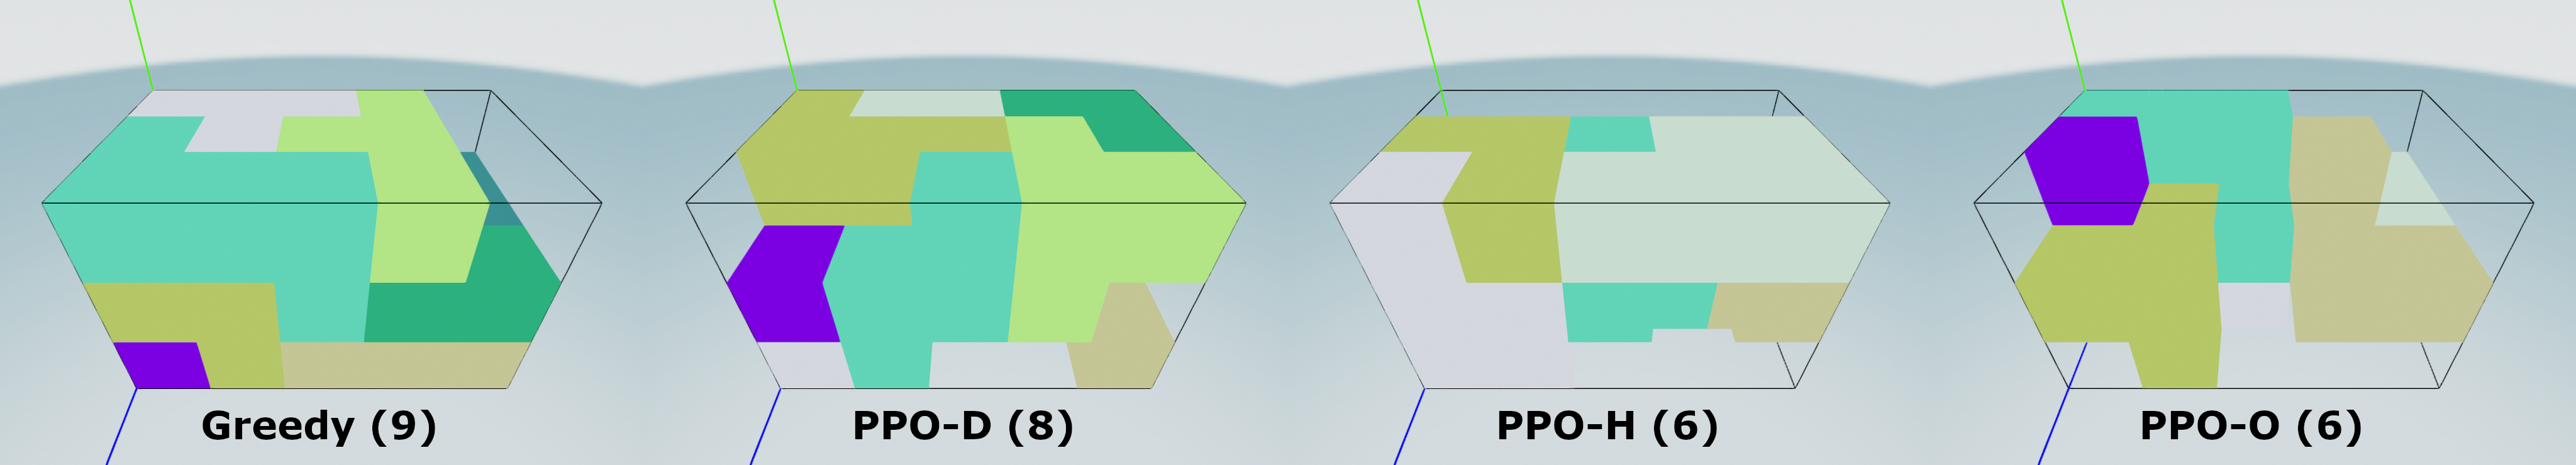
\includegraphics[scale=0.125]{images/vis-5x3x3-42.png}
    \caption{Packing on a $5 \times 3 \times 3$ container with a seed of 42.\label{fig:vis-5x3x3-42}}
\end{figure}

\begin{figure}[!htb]
    \centering
    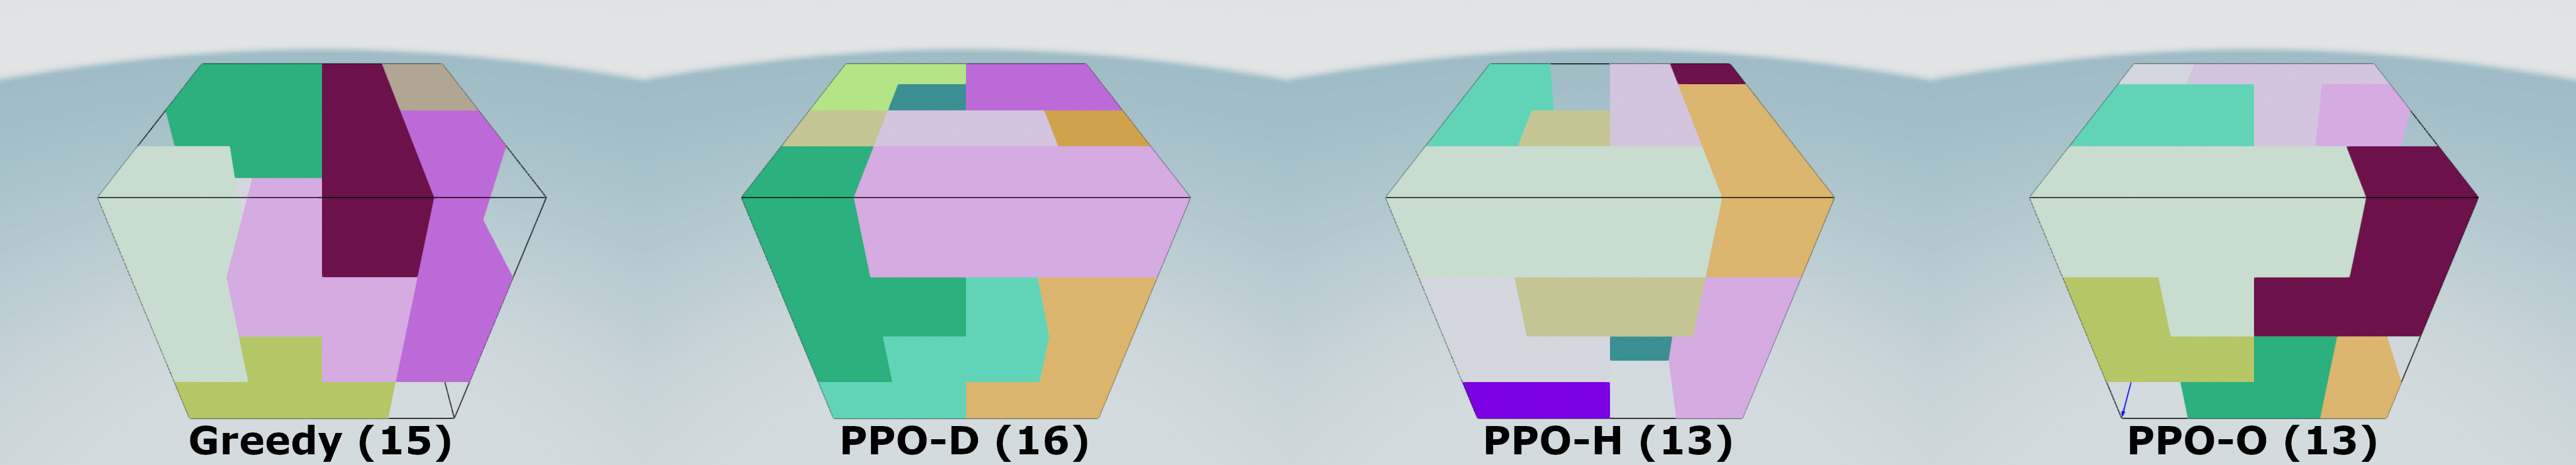
\includegraphics[scale=0.125]{images/vis-4x4x4-42.png}
    \caption{Packing on a $4 \times 4 \times 4$ container with a seed of 42.\label{fig:vis-4x4x4-42}}
\end{figure}

\begin{figure}[!htb]
    \centering
    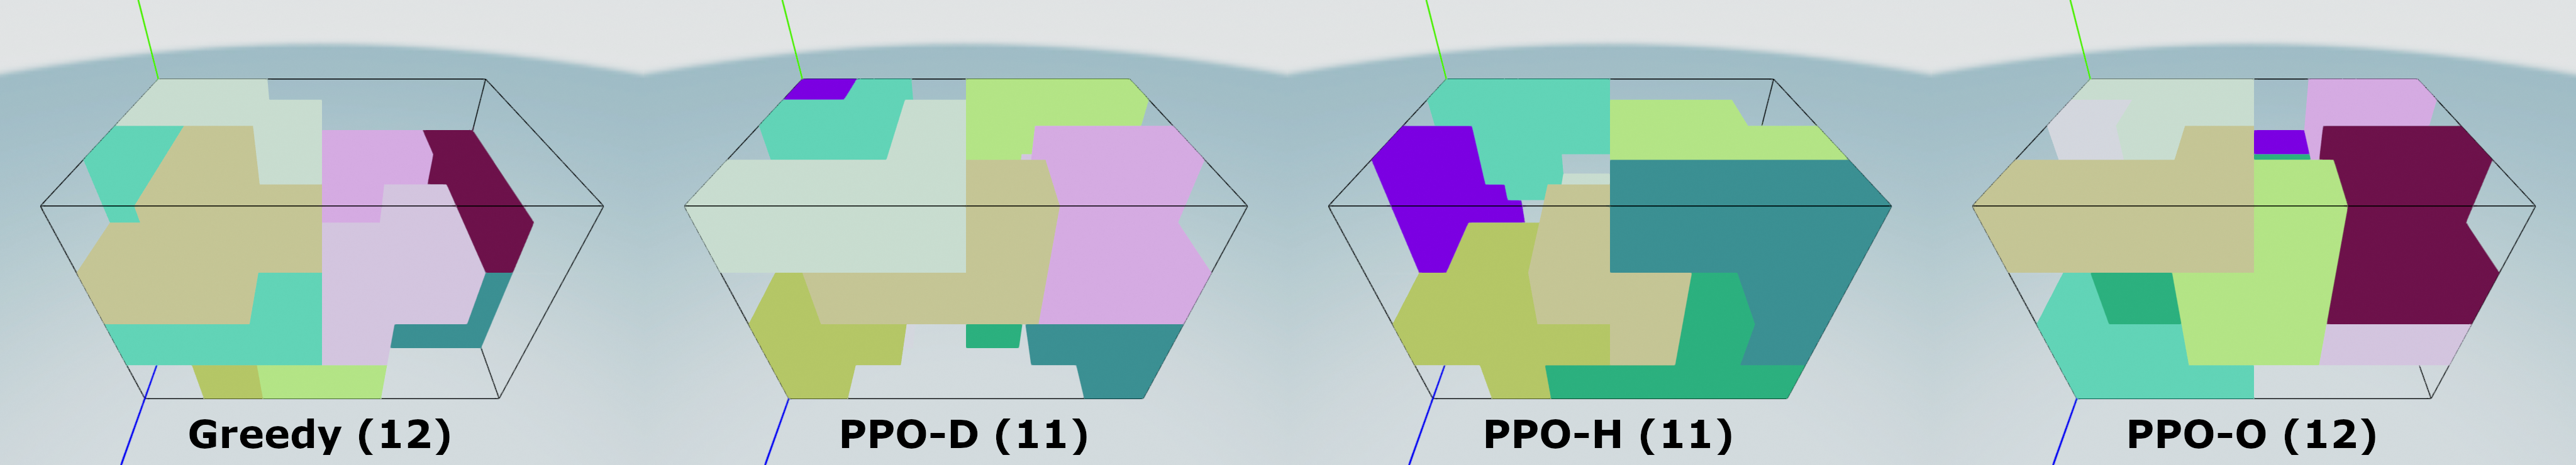
\includegraphics[scale=0.125]{images/vis-6x4x4-42.png}
    \caption{Packing on a $6 \times 4 \times 4$ container with a seed of 42.\label{fig:vis-6x4x4-42}}
\end{figure}

\begin{figure}[!htb]
    \centering
    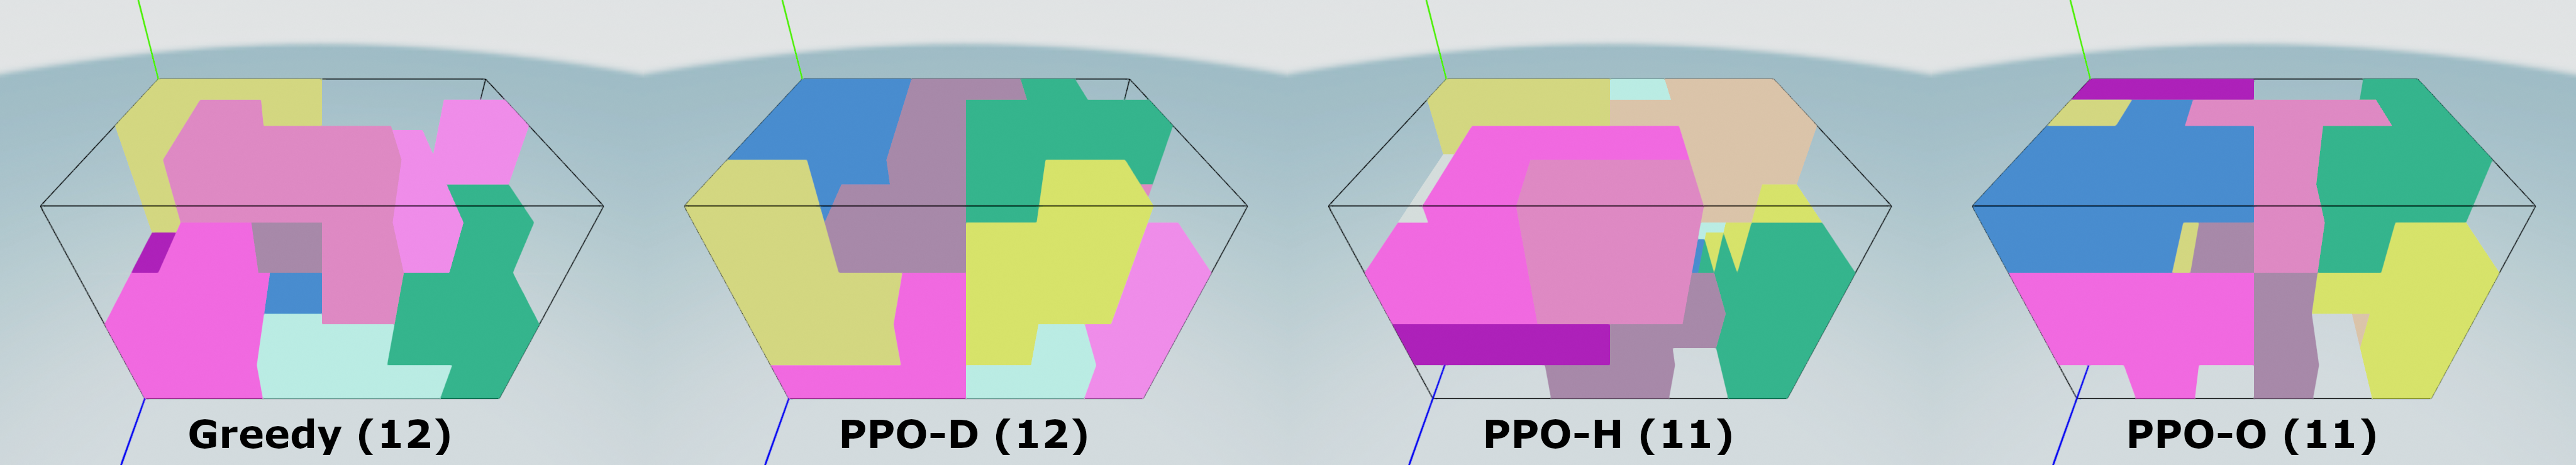
\includegraphics[scale=0.125]{images/vis-6x4x4-99.png}
    \caption{Packing on a $6 \times 4 \times 4$ container with a seed of 99.\label{fig:vis-6x4x4-99}}
\end{figure}

\end{document}
